% !TeX program = xelatex

%___________________________________________________________________
% Load Class

\documentclass[
  fontsize=10pt, 
  aspectratio=169,
  xcolor={dvipsnames}
]{beamer}
% beamer auto loads hyperref, color, xcolor, amsthm

%___________________________________________________________________
% Load Packages

% \usepackage[T1]{fontenc}        % * only if font supports T1 *
% \usepackage[utf8]{inputenc}     % * redundant for modern latex versions *

\usepackage{fontspec}               % required for system fonts
\usepackage{microtype}         % better typography
\usepackage{polyglossia}    % languages

% \usepackage{enumitem}

\usepackage{animate}

% citations
\usepackage[
  backend=biber,              
  style=ieee,                 
]{biblatex}   
\usepackage[
  autostyle=true, 
  german=quotes
]{csquotes}

% better unit display
\usepackage[
  locale=DE,
  mode=match,
  % per-mode-fraction,
  range-units=repeat,
  range-phrase={{~bis~}}
]{siunitx}

\usepackage{amsmath}

% input external data
\usepackage{listings}
\usepackage{graphicx} 
\usepackage{svg}

% improve visualization of data
\usepackage{booktabs}
\usepackage{tabularx}
\usepackage{longtable}
\usepackage{subcaption}	

\usepackage{appendixnumberbeamer}

\usetheme[]{metropolis}     % beamer style

%___________________________________________________________________
% Dimensions

\newlength{\imagewidth}
\setlength{\imagewidth}{1\columnwidth}

\newlength{\imageheight}
\setlength{\imageheight}{0.85\textheight}

%___________________________________________________________________
% Colors

\definecolor{colorblue}{HTML}{0480CC}				% color for weblinks
\definecolor{colordarkblue}{HTML}{4C1DCC}			% no use case at the moment
\definecolor{colorgreen}{HTML}{26CC1B}				% color for citations
\definecolor{colorred}{HTML}{CC1204}				% color for pdf links
\definecolor{coloryellow}{HTML}{F0B707}			    % color for warnings

%___________________________________________________________________
% New Makros

\newcommand{\imagesource}[1]{\par\footnotesize\textbf{Quelle:}~#1}   	%   Quellen für Bilder
\newcommand{\imagelegend}[1]{\par\footnotesize\textbf{Legende:}~#1}

\newcommand{\missing}{%
    \textcolor{coloryellow}{MISSING}%
    \PackageWarning{JHstyle}{You used the 'missing' macro at this line. Remove it before finalising document}%
}
\newcommand{\improve}{%
    \textcolor{coloryellow}{IMPROVE}%
    \PackageWarning{JHstyle}{You used the 'improve' macro at this line. Remove it before finalising document}%
}

%___________________________________________________________________
% Renamings

\renewcommand{\lstlistingname}{Quellcode}						%	Snippet umbenennen
\renewcommand{\lstlistlistingname}{Codeverzeichnis}	

\addto\captionsgerman{%
  \renewcommand{\proofname}{Beweis}
}

\renewcommand{\mkcitation}[1]{#1}

%___________________________________________________________________
% Commands

\setdefaultlanguage{german}
\setotherlanguage{english}

\addbibresource{sources.bib}

\graphicspath{{images/}}  

\hypersetup{
%   hidelinks,
  colorlinks=true,
  linkcolor=.,
  anchorcolor=.,
  % citecolor=green,
  % filecolor=magenta,      
  urlcolor=colorblue,
  bookmarksnumbered=true,
  breaklinks=true,
  pdfauthor=Jan Hoegen,
  pdftitle=Pytorch NNB
}

%___________________________________________________________________
% Listings

\lstset{%
	frame			=	tb ,							%	horizontale Linie oben&unten
	breaklines		=	true,							%	Zeilenumbruch
	rulecolor		=	\color{black} ,					%	Rahmenfarbe ist schwarz
	keywordstyle	=	\color{colorblue} ,
	commentstyle	=	\color{colorblue} ,
	stringstyle		=	\color{colorblue} ,
	title			=	\lstname ,						%	Titel ist gleich dem Dateinamen
	basicstyle		=	\footnotesize\ttfamily ,		%	Kleine Schrift und Monospace
	numbers			=	left,							%	Zeilennumber links
	inputencoding	=	utf8,  							% Input encoding
  extendedchars	=	true,  							% Extended ASCII
}

%___________________________________________________________________
% Ttile Page

\title{CIFAR10 mit PyTorch klassifizieren}
\subtitle{Neuronale Netze in der Bildverarbeitung}
\date{\today}
\author{Jan Hoegen \and Nico Weber}
\institute{
  Hochschule Karlsruhe\\
  University of Applied Sciences
}
% \setbeamertemplate{frame footer}{CIFAR10 mit PyTorch klassifizieren. Jan Hoegen, Nico Weber}

%___________________________________________________________________
% Document

\begin{document}
  \maketitle

  \begin{frame}{Inhaltsverzeichnis}
    \setbeamertemplate{section in toc}[sections numbered]
    \tableofcontents[hideallsubsections]
    % \tableofcontents
  \end{frame}

  \section{Allgemeines zu Pytorch}

\begin{frame}{PyTorch im Überblick}
    \begin{columns}[T,onlytextwidth]
        \column{0.5\textwidth}
        
        Was ist Pytorch
        \begin{itemize}
            \item Python Library für Deep Learning
            \item Beliebt in Forschung und Lehre \cite{bauer}
        \end{itemize}

        \column{0.5\textwidth}
        Warum Pytorch
        \begin{itemize}
            \item Einfache und flexible Modell-Implementierung
            \item Direkte Nutzung von GPU-Beschleunigung
            \item Große Community und viele Tutorials
        \end{itemize}
    \end{columns}
\end{frame}

%___________________________________________________________________

\begin{frame}{Grundlegende Konzepte}
    \begin{description}
        \item[Auto Gradient] Backpropagation wird automatisch berrechnet 
        \item[nn.Module] Vordefinierte Layers
        \item[Data Loader] Einfaches Laden und \alert{Parallelisieren} der Datensätze
        \item[Optimizer] Hinterlegte Optimierfunktionen, z.B. Adam   
    \end{description}
    
\end{frame}


  \section{Eigenes Modell zu CIFAR 10}

%___________________________________________________________________

\begin{frame}{Aufgabenstellung}
    \begin{itemize}[left=1em] % optional: Einzug leicht verringert
        \item \textbf{Aufgabe:} Klassifikation von CIFAR-10 Bildern
        \item \textbf{Datensatz:}
            \begin{itemize}[topsep=1pt, itemsep=1pt] % engerer Abstand für Unterpunkte
                \item 60.000 Bilder, 10 Klassen, Größe $32\times32\times3$
                \item Trainingsset: 49.000 Bilder
                \item Validierungsset: 1.000 Bilder
                \item Testset: 10.000 Bilder
            \end{itemize}
        \item \textbf{Ziel:} Modell in \emph{maximal 10 Epochen} trainieren, um Bilder korrekt zu klassifizieren
    \end{itemize}
\end{frame}



%___________________________________________________________________

\begin{frame}{Architektur des Modells}
    \begin{figure}
        \centering
        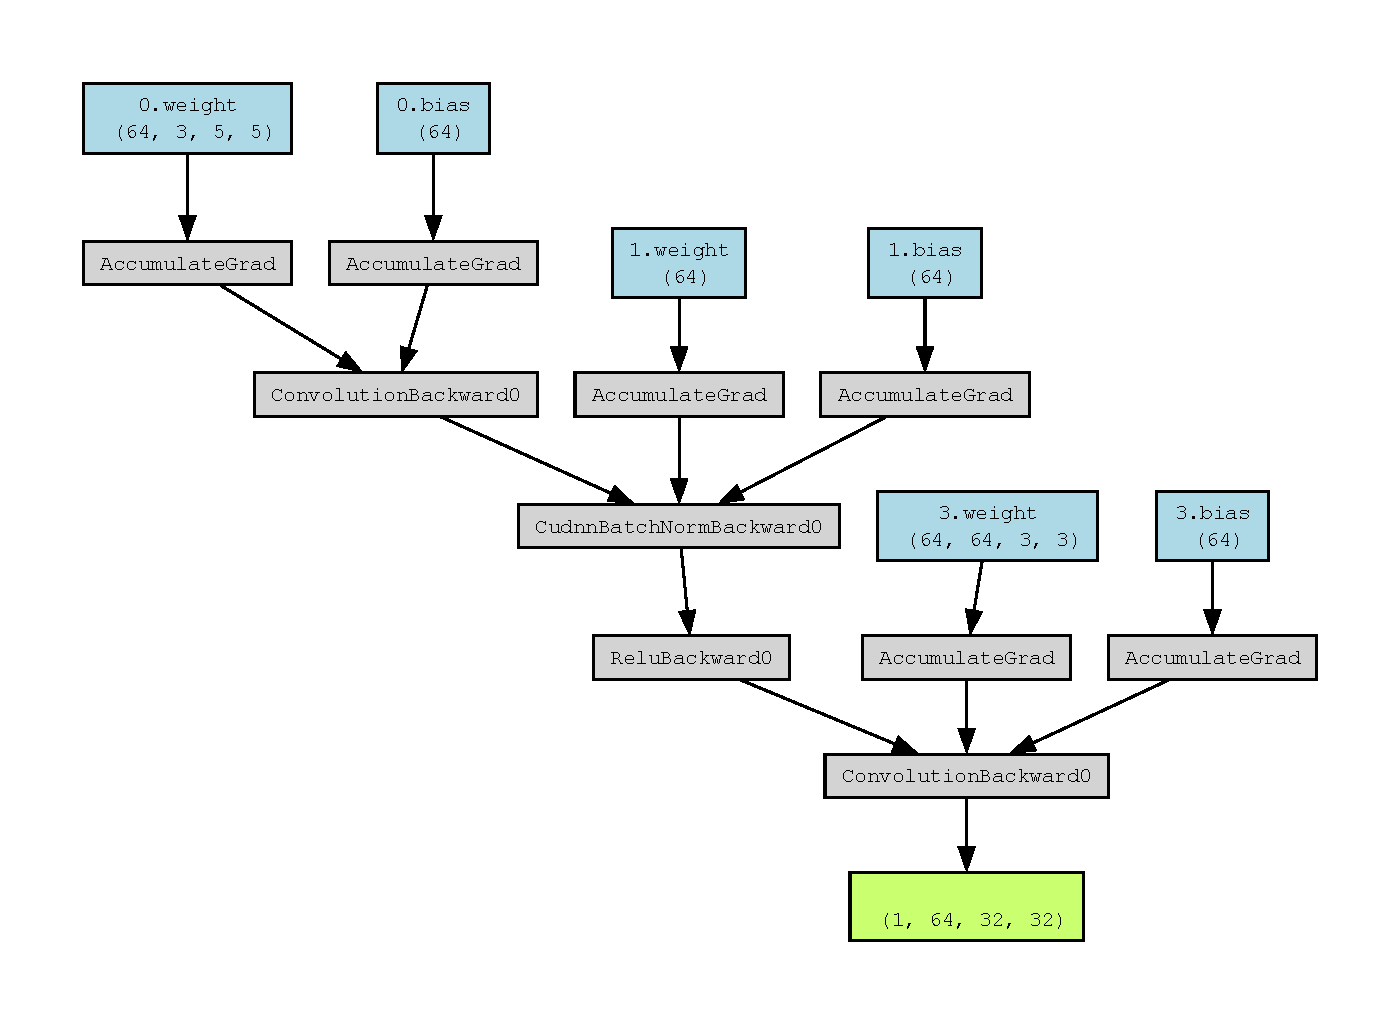
\includegraphics[width=\imagewidth, height=\imageheight, keepaspectratio]{reduced_graph.pdf}
    \end{figure}

\end{frame}

%___________________________________________________________________

\begin{frame}{Ergebnisse des besten Modells}

\begin{description}
    \item[Gewählte Hyperparameter:]
        \begin{itemize}
            \item ch1 = 64, ch2 = 64, ch3 = 64
            \item Lernrate = 0.00086
            \item Weight Decay = 3.81e-6
        \end{itemize}

    \item[Best Validation Accuracy:] \alert{75.70\%}
    
    \item[Trainings-Accuracy:] \alert{73\%}

    \item[Test Accuracy:] \alert{75.05\%}
\end{description}
\end{frame}

%___________________________________________________________________

\begin{frame}{Accuracy für verschiedene Klassen}
    \begin{figure}
        \centering
        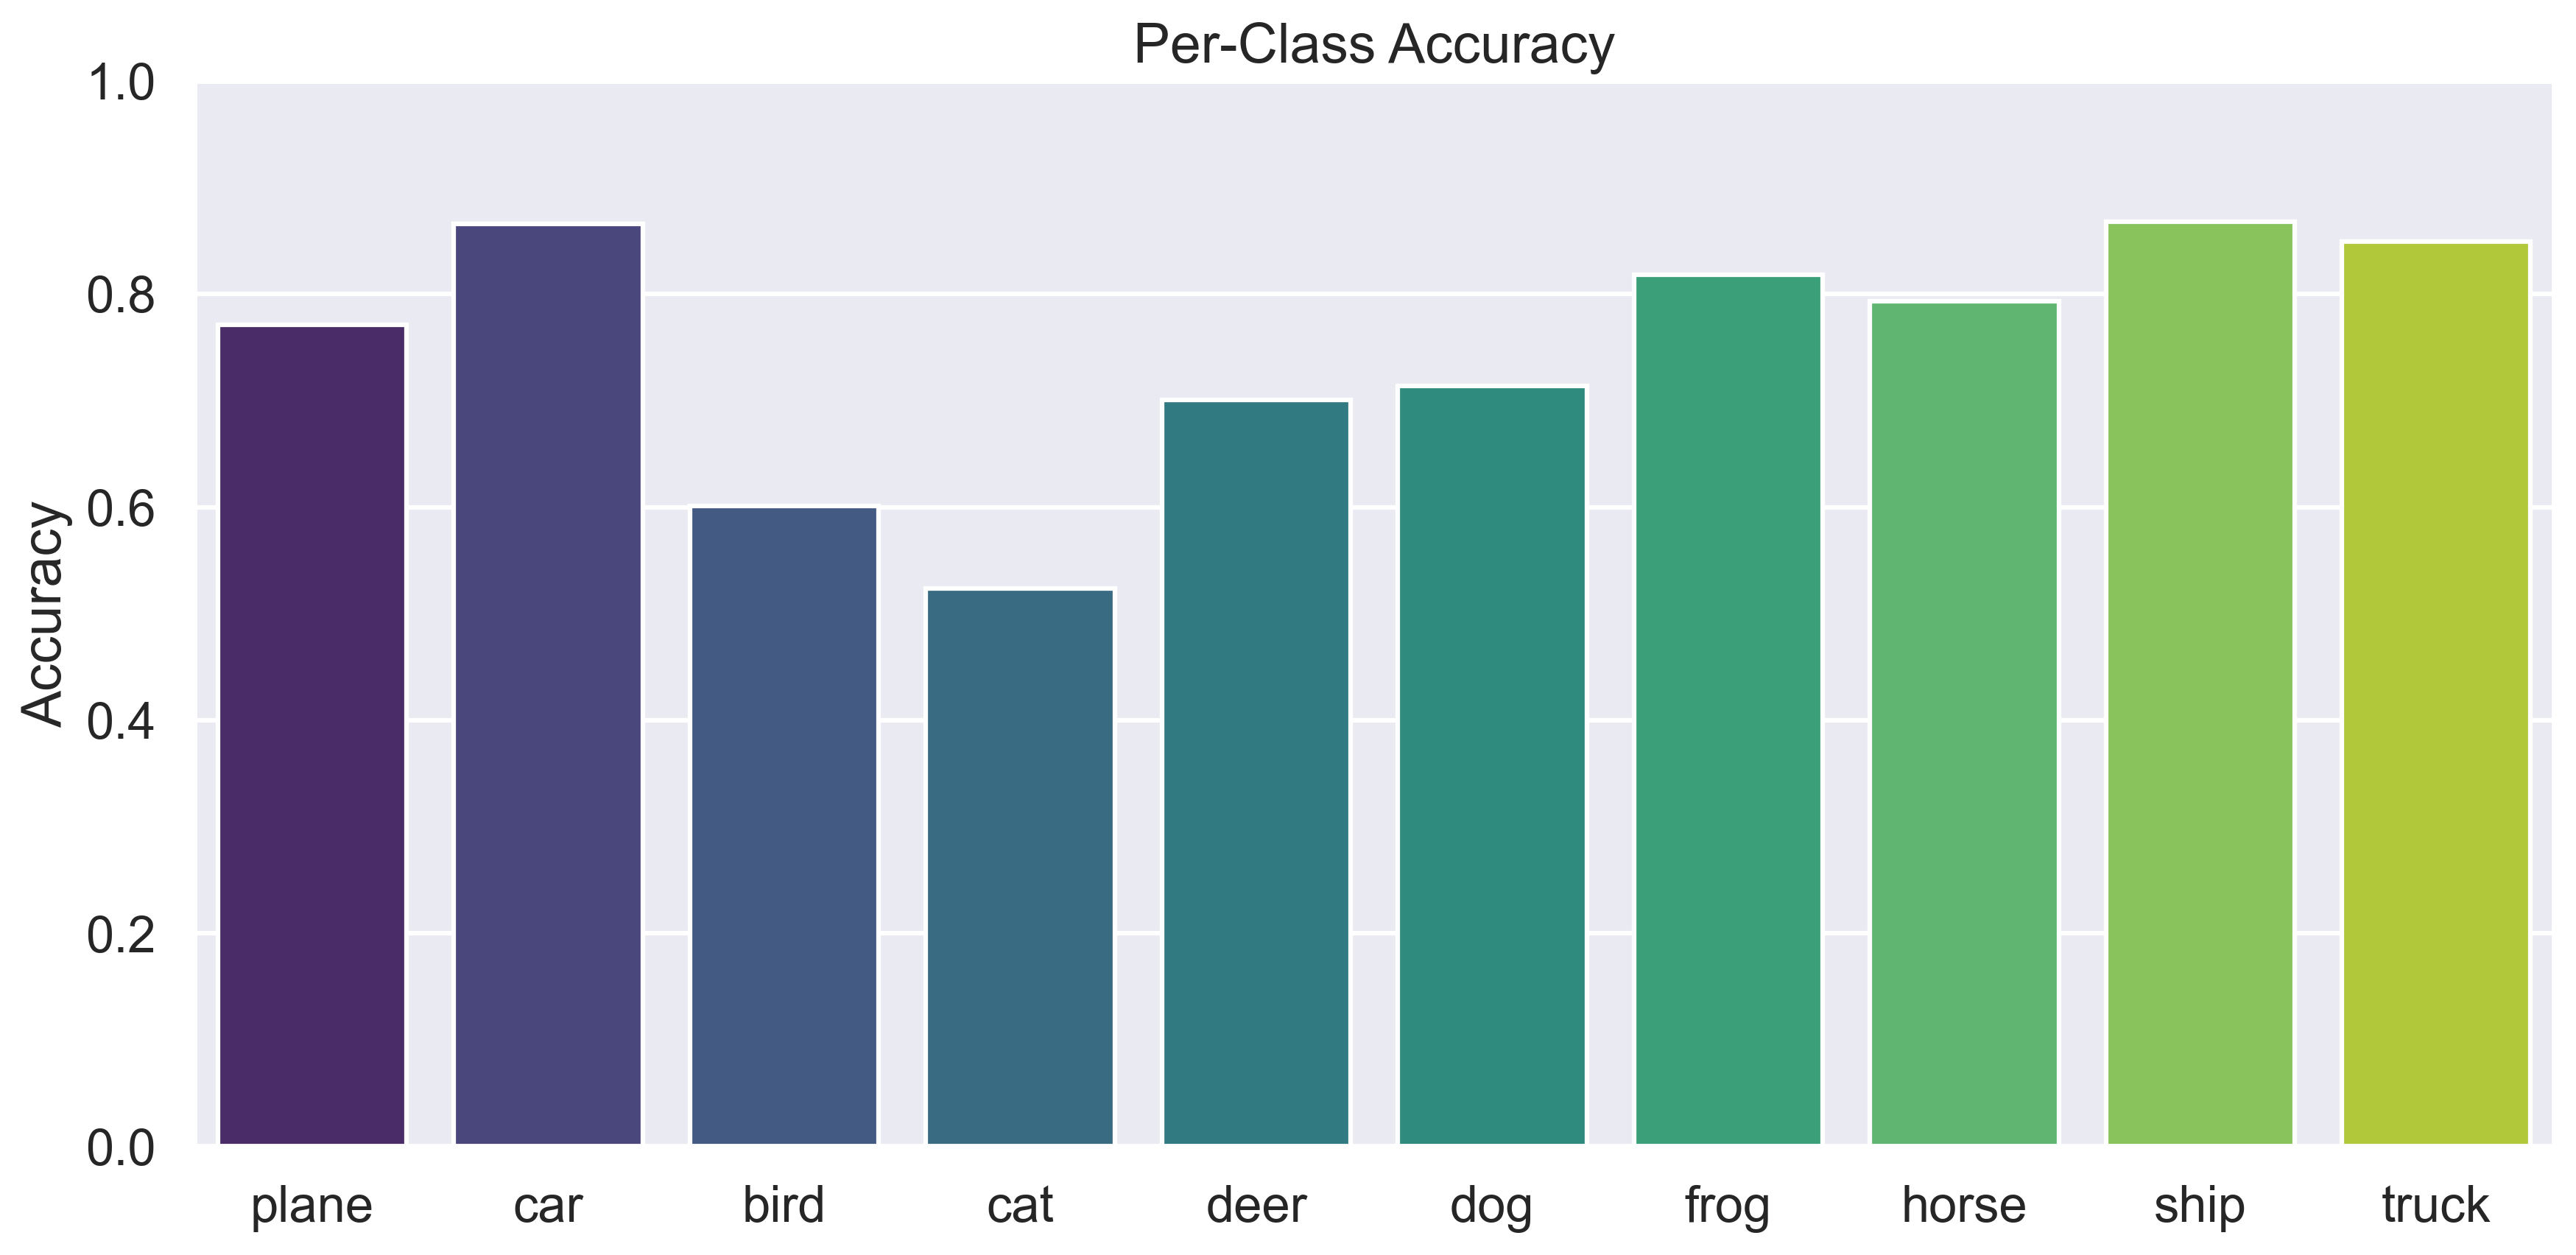
\includegraphics[width=\imagewidth, height=\imageheight, keepaspectratio]{class_accuracy.png}
    \end{figure}
\end{frame}

%___________________________________________________________________

\begin{frame}{Confusion Matrix}
    \begin{figure}
        \centering
        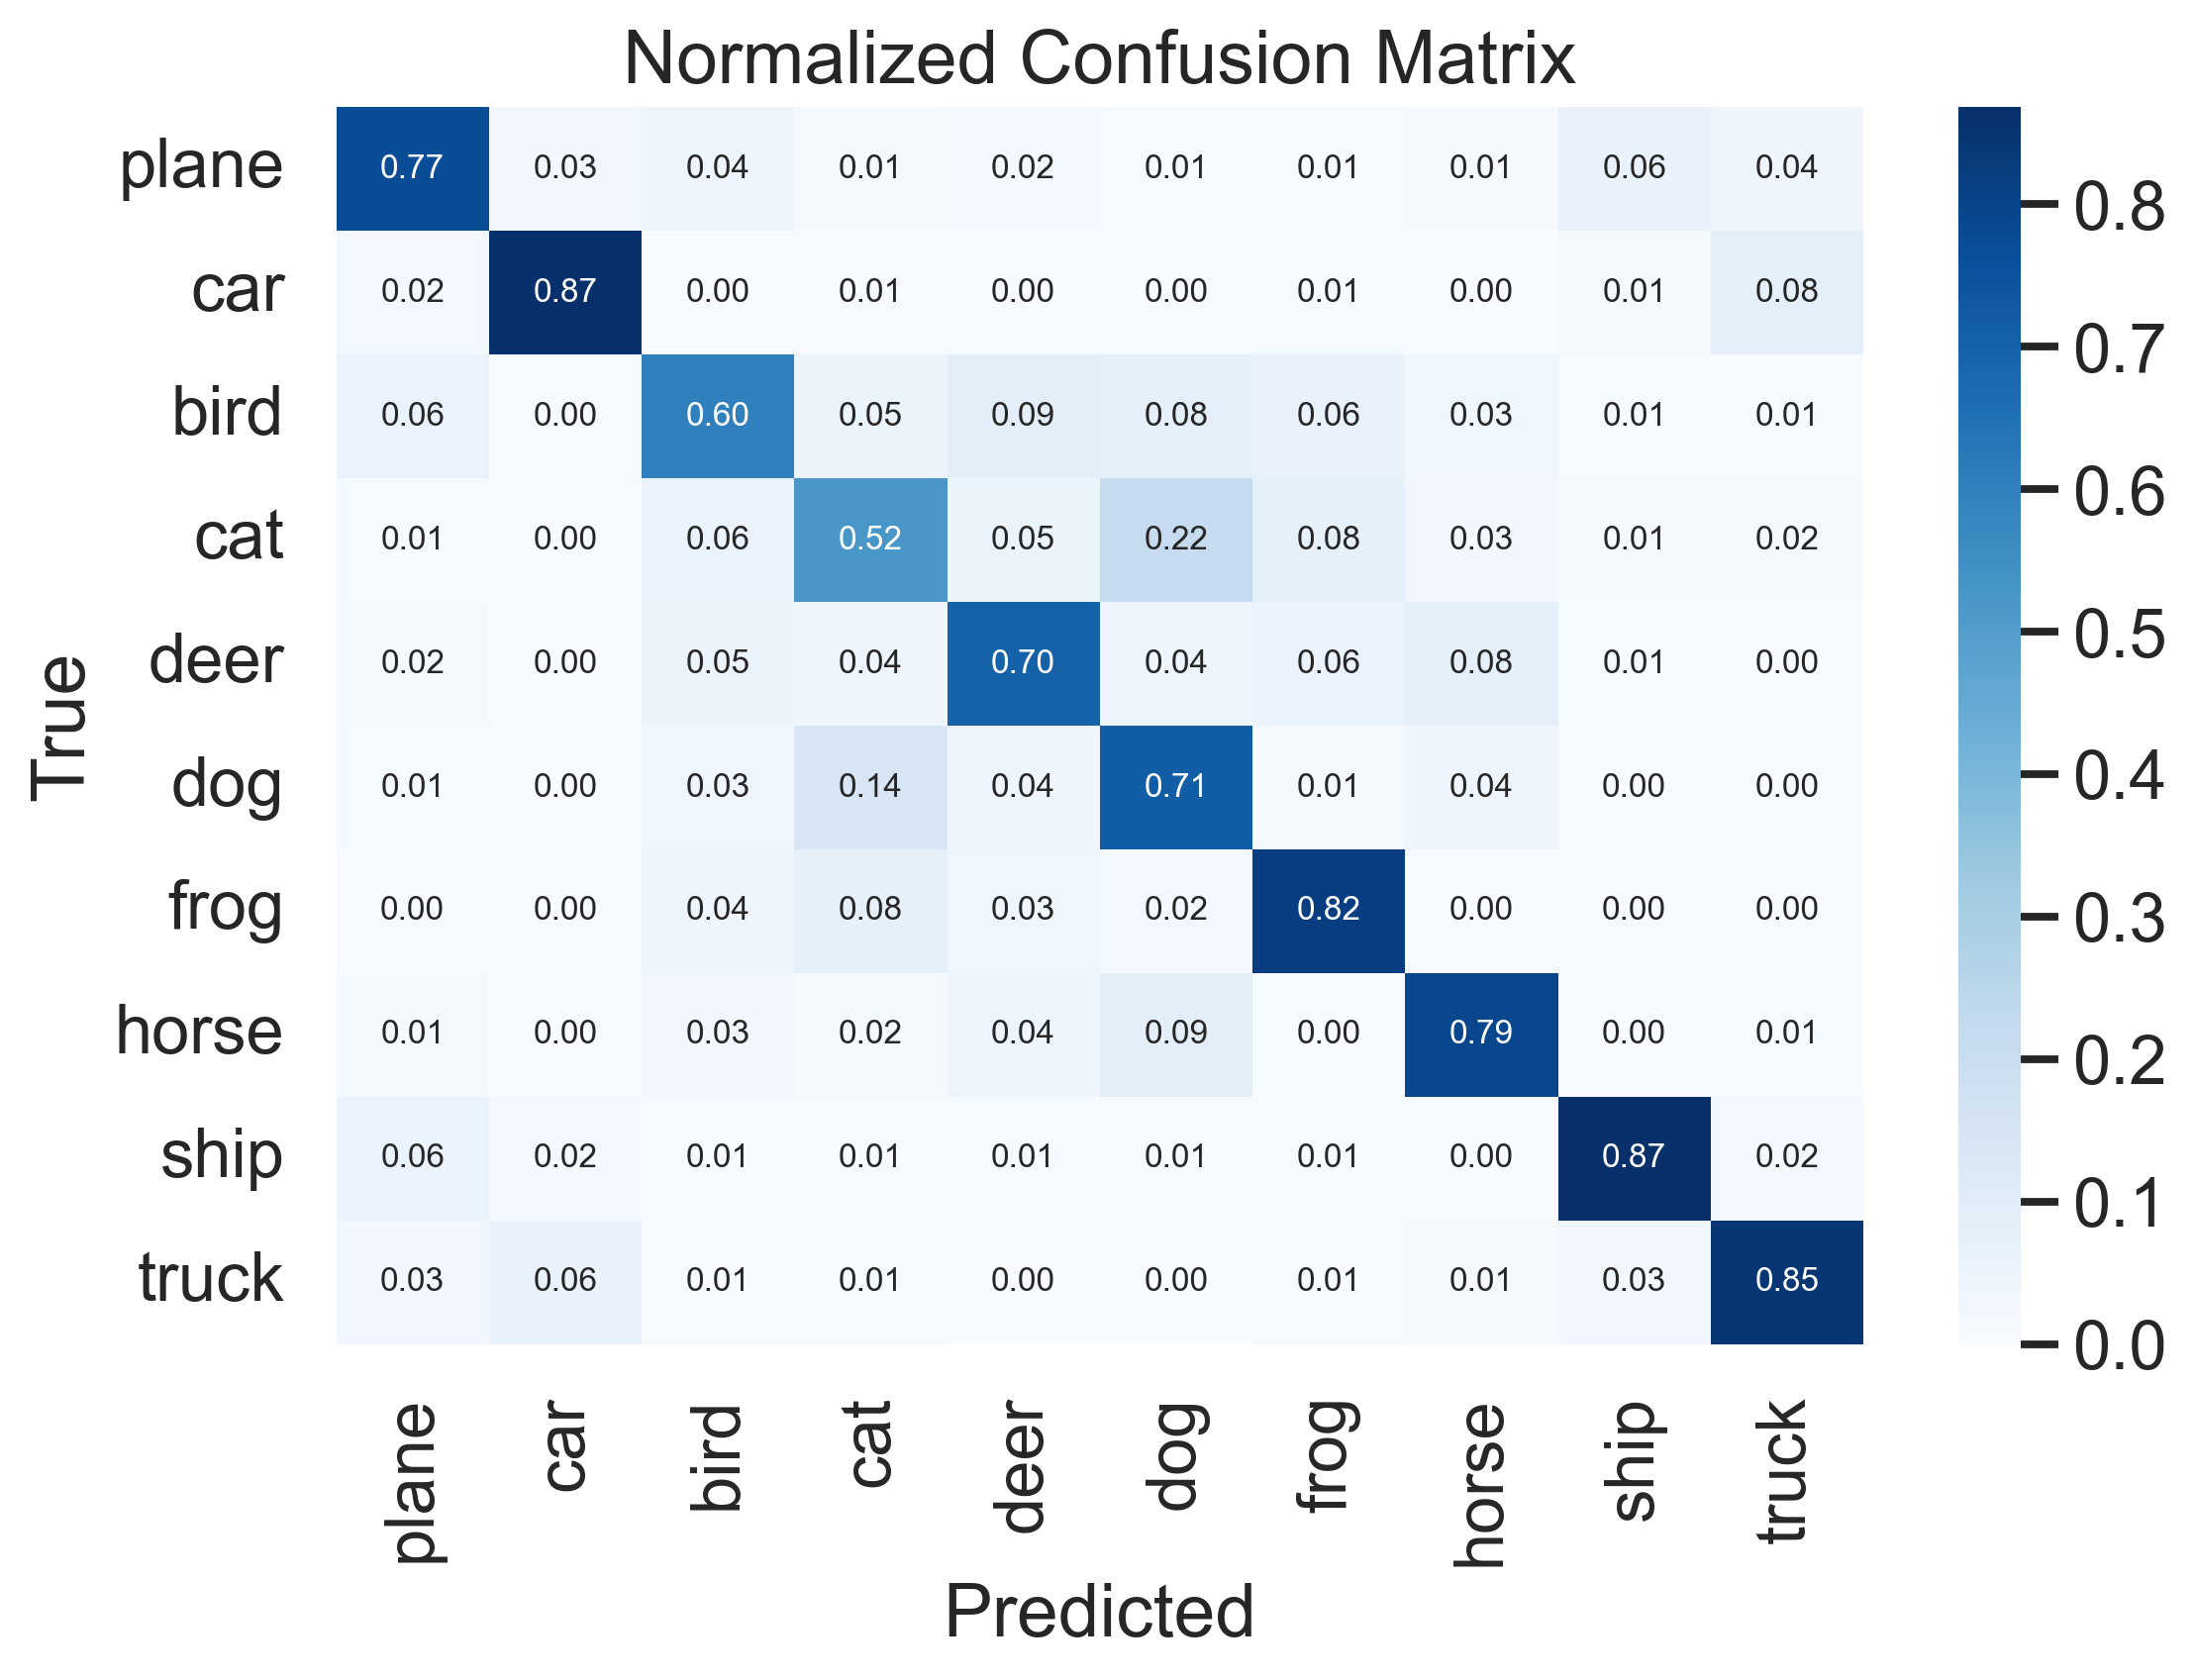
\includegraphics[width=\imagewidth, height=\imageheight, keepaspectratio]{confusion_matrix.png}
    \end{figure}
\end{frame}

%___________________________________________________________________

\begin{frame}{Beispielbilder}
    \begin{figure}
        \centering
        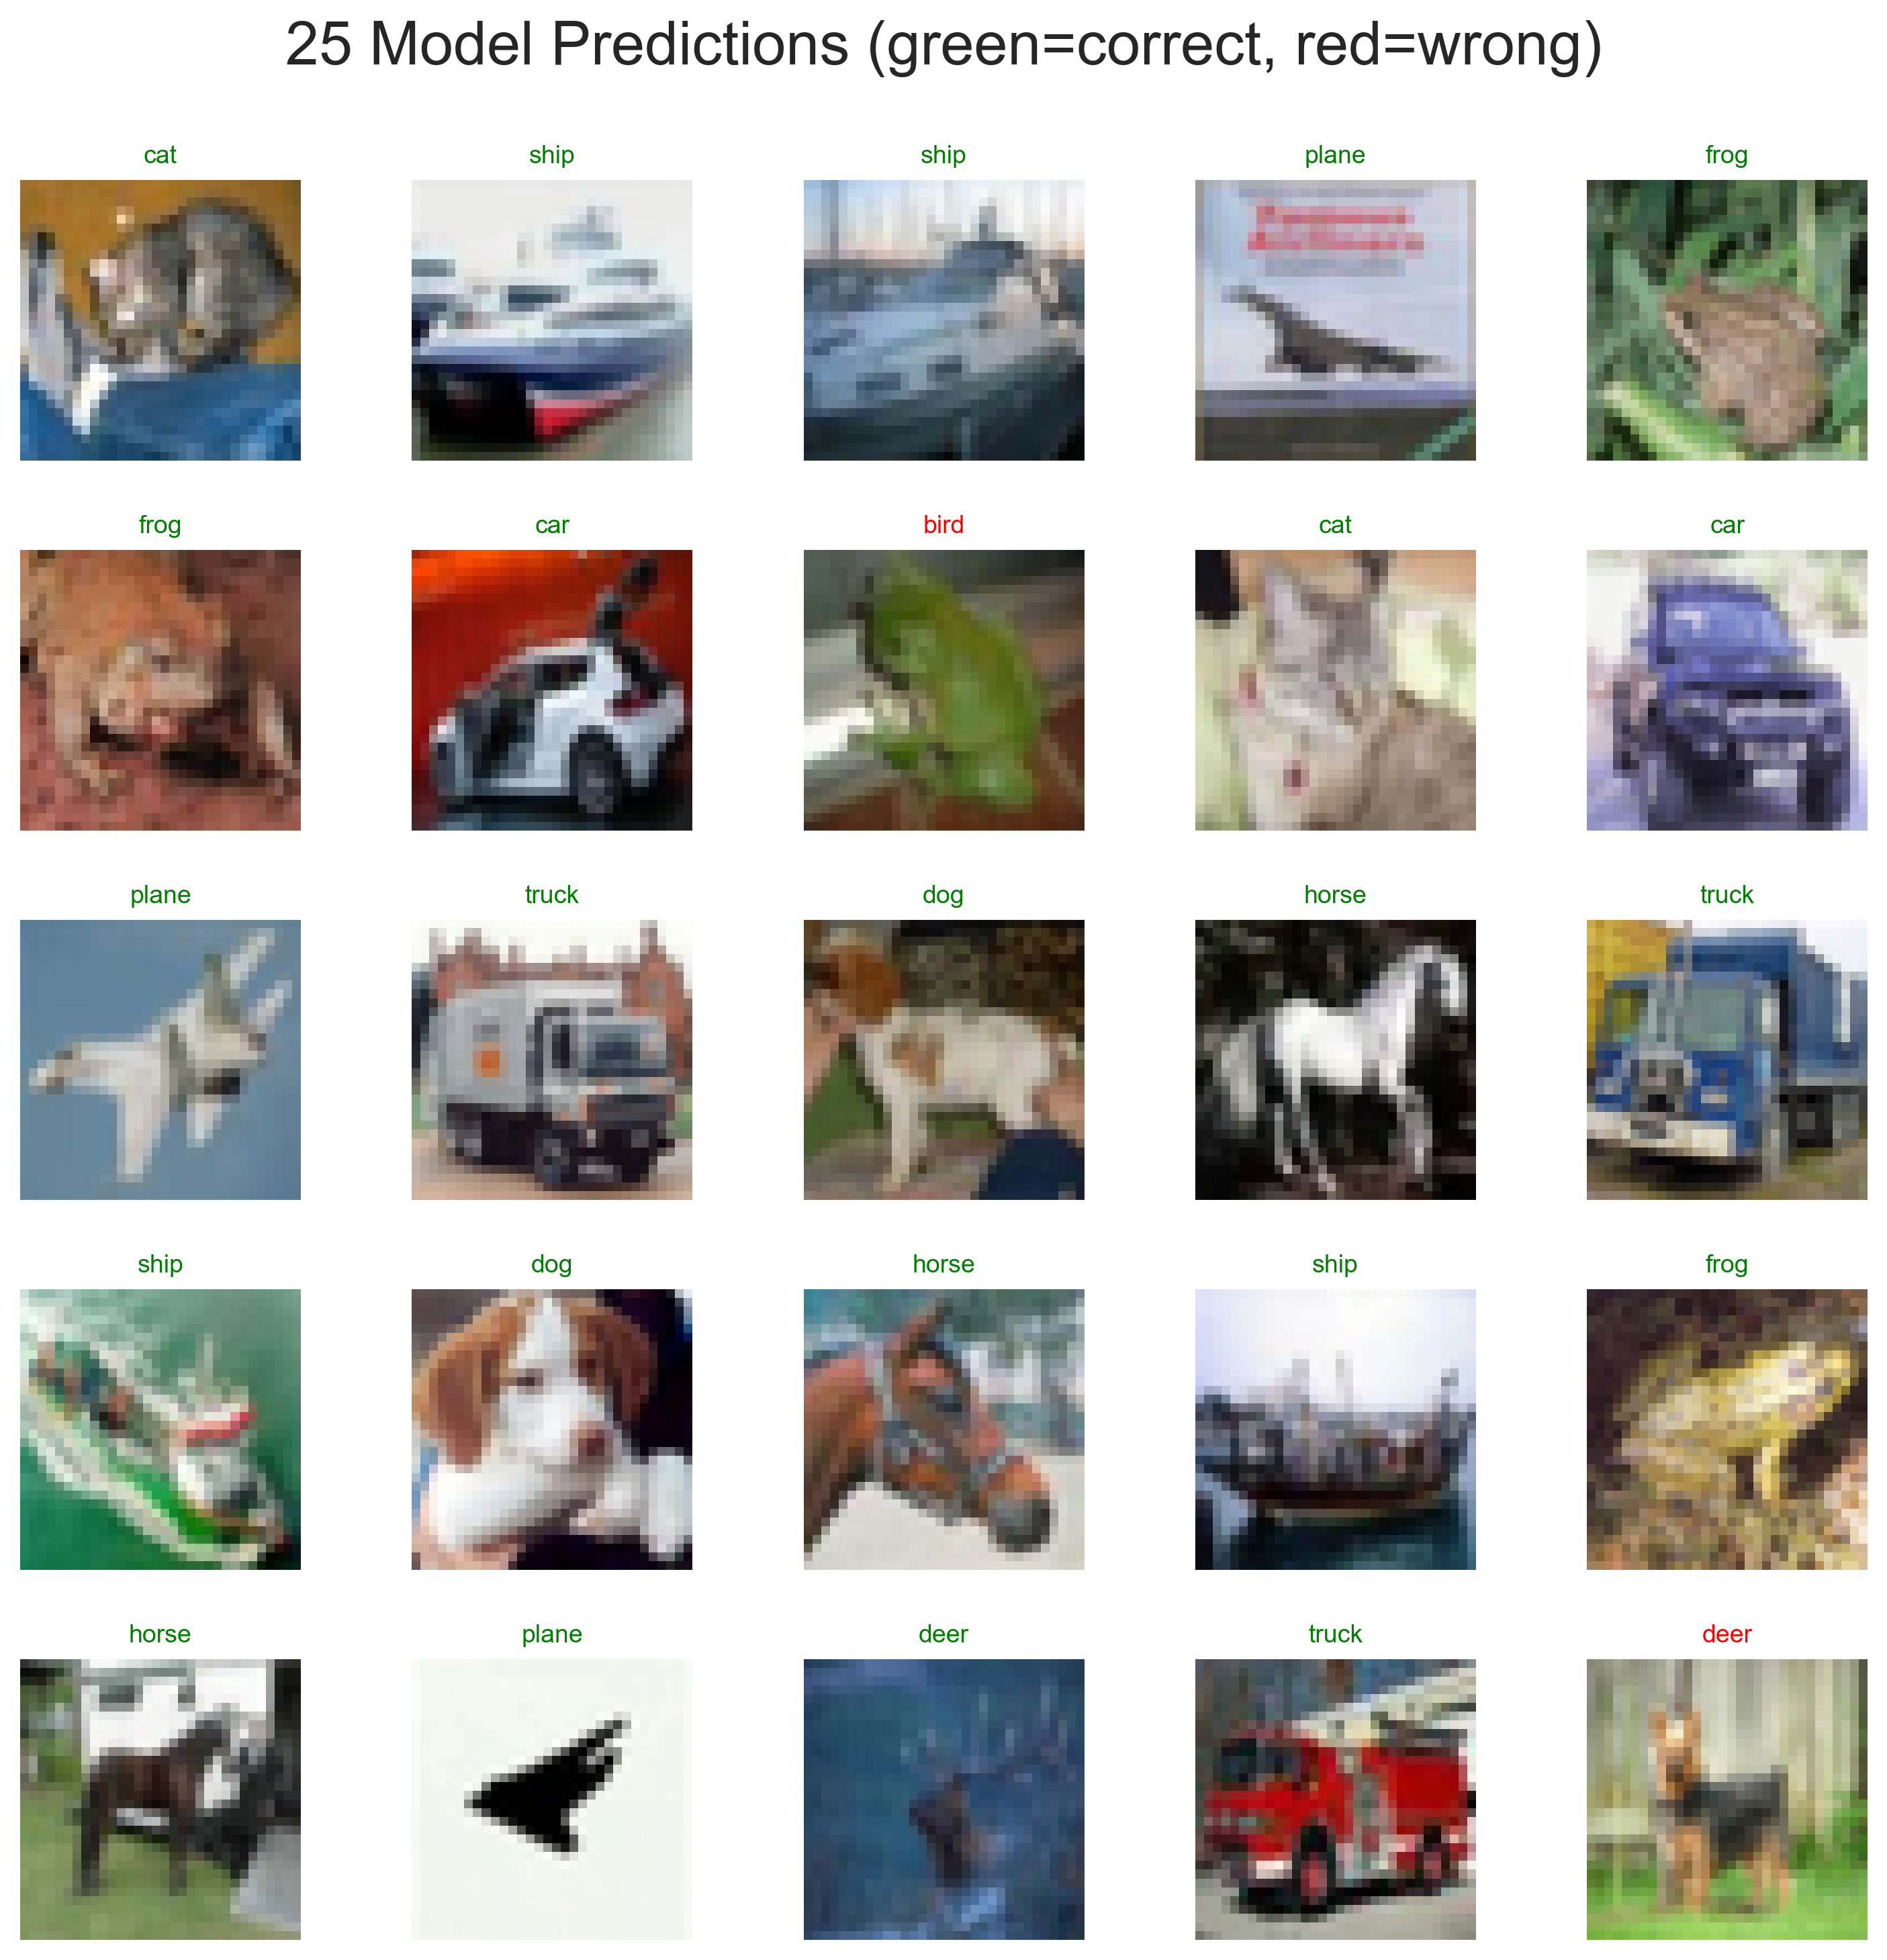
\includegraphics[width=\imagewidth, height=\imageheight, keepaspectratio]{predictions_grid.png}
    \end{figure}
\end{frame}



  \section{Training und Hyperparameter}

%___________________________________________________________________
\begin{frame}{Einstellungen für das Training}

\textbf{Trainingsdaten:}
\begin{itemize}
    \item 49.000 Trainingsbilder, Größe $32 \times 32 \times 3$
    \item Batchgröße: 256
    \item DataLoader-Worker: 12 (hohe Parallelisierung)
\end{itemize}

\textbf{Training:}
\begin{itemize}
    \item Trainierbare Parameter: 604 810
    \item Iterationen pro Epoche: $\lceil 49{,}000 / 256 \rceil = 192$
    \item Epochen je Hyperparameter-Kombination: 10
\end{itemize}

\textbf{Hyperparameter-Optimierung:}
\begin{itemize}
    \item \alert{Bayesian Search} mit 20 Hyperparameter-Kombinationen (Trials)
    \item Optimierte Parameter: ch1, ch2, ch3, Lernrate, Weight Decay
\end{itemize}
\end{frame}

%___________________________________________________________________
\begin{frame}{Genauigkeit während des Trainings}
\begin{figure}
    \centering
    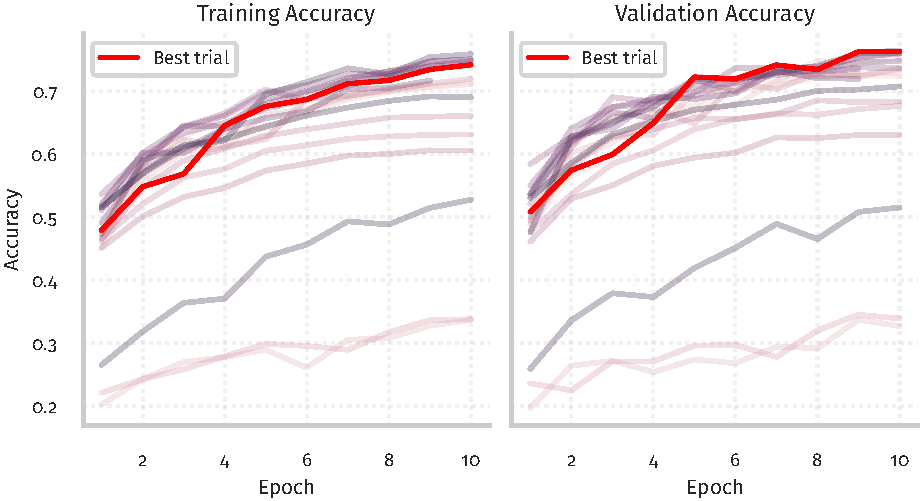
\includegraphics[width=\imagewidth, height=\imageheight, keepaspectratio]{all_trials_accuracy.pdf}
    \caption{Validation und Training für verschiedene Traials.}
\end{figure}
\end{frame}

%___________________________________________________________________
\begin{frame}[fragile]{Early Stopping}
\textbf{Motivation:} 
\begin{itemize}
    \item Verhindert Overfitting
    \item Stoppt das Training, wenn die Validierungsgenauigkeit über mehrere Epochen nicht steigt
\end{itemize}

\textbf{Prinzip:}
\begin{itemize}
    \item Lege Grenzwert \texttt{patience} fest
    \item Nach jeder Epoche: Bestwert der Validierungsgenauigkeit speichern
    \item Zähle Epochen ohne Verbesserung: \texttt{epochs\_no\_improvement}
    \item Bei neuer Verbesserung: Zähler \texttt{epochs\_no\_improvement} zurücksetzen
    \item Stoppe Training, sobald \texttt{epochs\_no\_improvement $\ge$ patience}
\end{itemize}
\end{frame}
%___________________________________________________________________
\begin{frame}{Hardware-Auslastung}
\begin{columns}[T,onlytextwidth]

    \column{0.45\textwidth}
    \textbf{Hardware:}
    \begin{itemize}
        \item GPU: RTX 4060 Ti, 16 GB VRAM
        \item CPU: Ryzen 5 7600X, 12 Kerne
        \item RAM: 32 GB DDR5
    \end{itemize}

    \column{0.55\textwidth}
    \begin{figure}
        \centering
        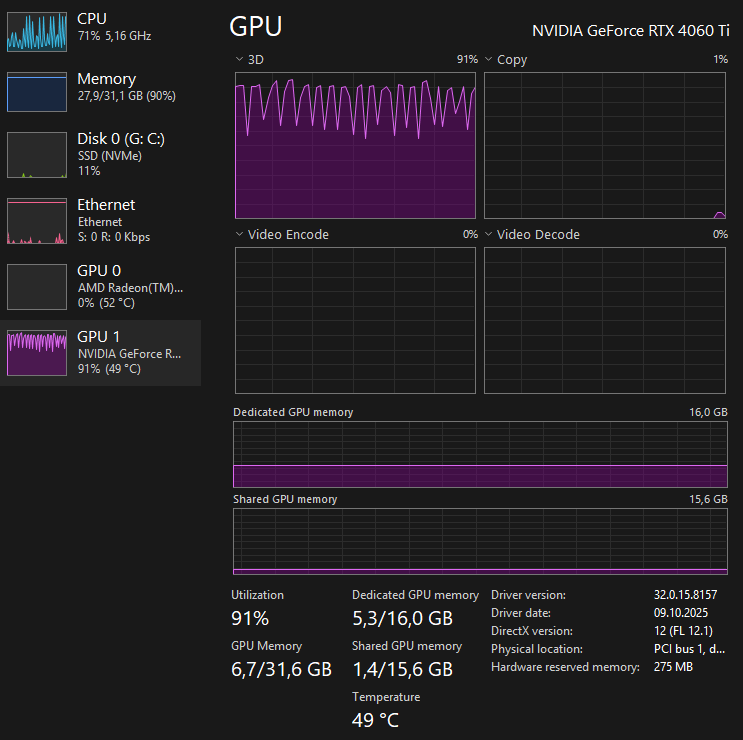
\includegraphics[width=\linewidth, height=0.8\textheight, keepaspectratio]{machine.png}
        \caption{Auslastung gemäß Task Manager}
    \end{figure}

\end{columns}
\end{frame}


%___________________________________________________________________
\begin{frame}{Laufzeiten pro Trial}
Gesamtdauer: ca. 15 Minuten

\begin{figure}
    \centering
    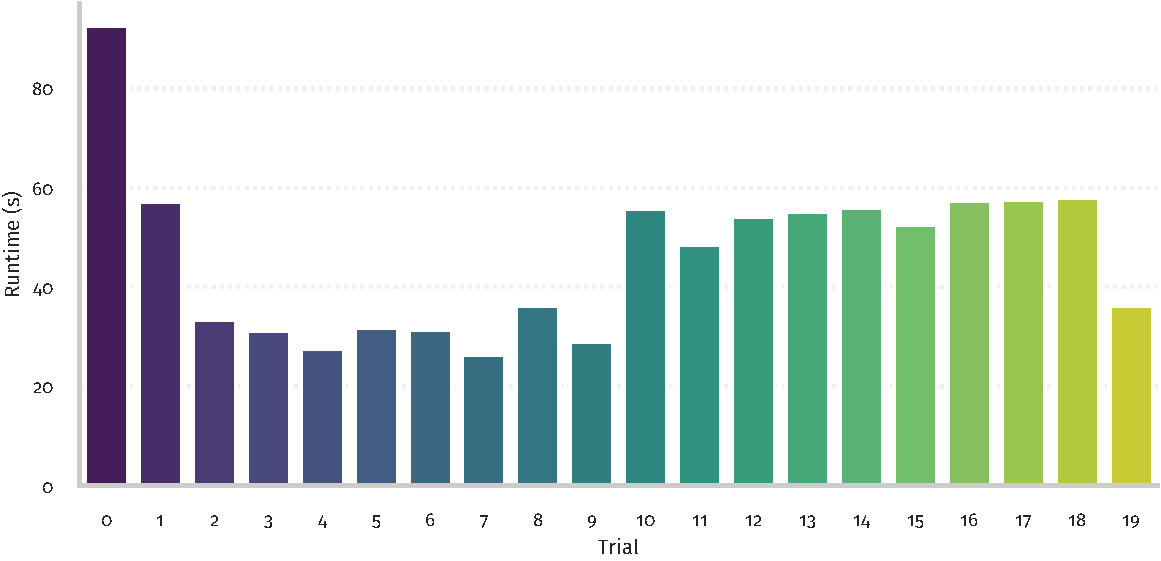
\includegraphics[width=\imagewidth, height=0.8\imageheight, keepaspectratio]{runtime_per_trial.pdf}
    \caption{Laufzeit des Trainings je Trial.}
\end{figure}
\end{frame}


  \section{Hyperparameter mit Bayesian Search}

%___________________________________________________________________
\begin{frame}{Bayesian Search Erklärt}
\begin{itemize}
    \item Bayesian Search ist eine intelligente Methode zur Optimierung von Hyperparametern.
    \item Ziel: Maximierung der Validierungsgenauigkeit $f(\text{Parameter}) \rightarrow \text{Validation Accuracy}$.
    \item Idee:
        \begin{itemize}
            \item Es wird ein Modell erstellt, das die unbekannte Zielfunktion $f$ abschätzt.
            \item Nach jeder Evaluierung wird dieses Modell mit den neuen Ergebnissen aktualisiert.
            \item Eine \textit{Acquisition Function} wählt die nächsten Parameterwerte aus – als Kompromiss zwischen \textbf{Exploration} (neue Bereiche testen) und \textbf{Exploitation} (bestehende gute Bereiche verfeinern).
        \end{itemize}
    \item Vorteil: Findet gute Parameter mit deutlich weniger Versuchen als Random oder Grid Search.
\end{itemize}
\end{frame}

%___________________________________________________________________
\begin{frame}{Animation zu Bayesian Search}
\centering
\animategraphics[loop, autoplay, controls, width=\imagewidth, height=\imageheight, keepaspectratio]{0.5}{videos/frame_}{000}{006}
\imagesource{\cite{bayes_gif}}
\end{frame}

%___________________________________________________________________
\begin{frame}{Anwendung auf unser Modell}
\begin{columns}[T,onlytextwidth]
    \begin{column}{0.52\textwidth}
        \begin{itemize}
            \item Anstatt zufällig Parameterkombinationen zu testen (Random Search) oder alle möglichen Kombinationen (Grid Search), wurde \textbf{Bayesian Search} verwendet.
            \item Das Modell der Funktion $\text{Validation Accuracy} = f(\text{Hyperparameter})$ wird kontinuierlich angepasst.
            \item Neue Vorschläge für Hyperparameter werden auf Basis bisheriger Ergebnisse erzeugt.
        \end{itemize}
    \end{column}
    \begin{column}{0.45\textwidth}
        \begin{figure}
            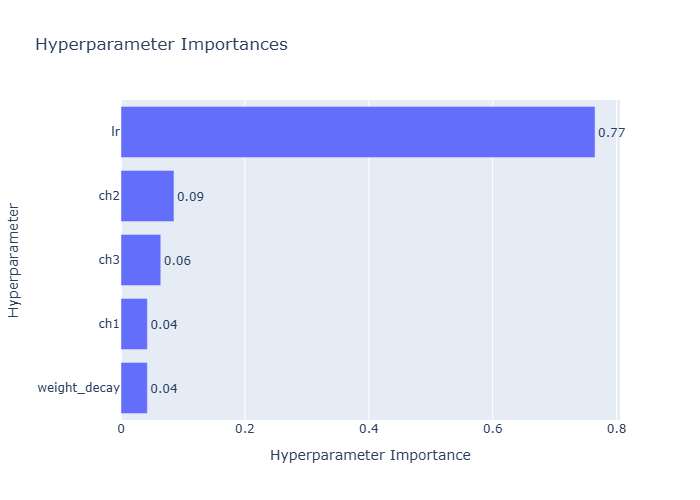
\includegraphics[width=\linewidth, height=\imageheight, keepaspectratio]{param_importances.png}
            \caption{Relative Wichtigkeit der Hyperparameter}
        \end{figure}
    \end{column}
\end{columns}
\end{frame}

%___________________________________________________________________
\begin{frame}{Bayesian Search Ergebnisse}
\begin{figure}
    \centering
    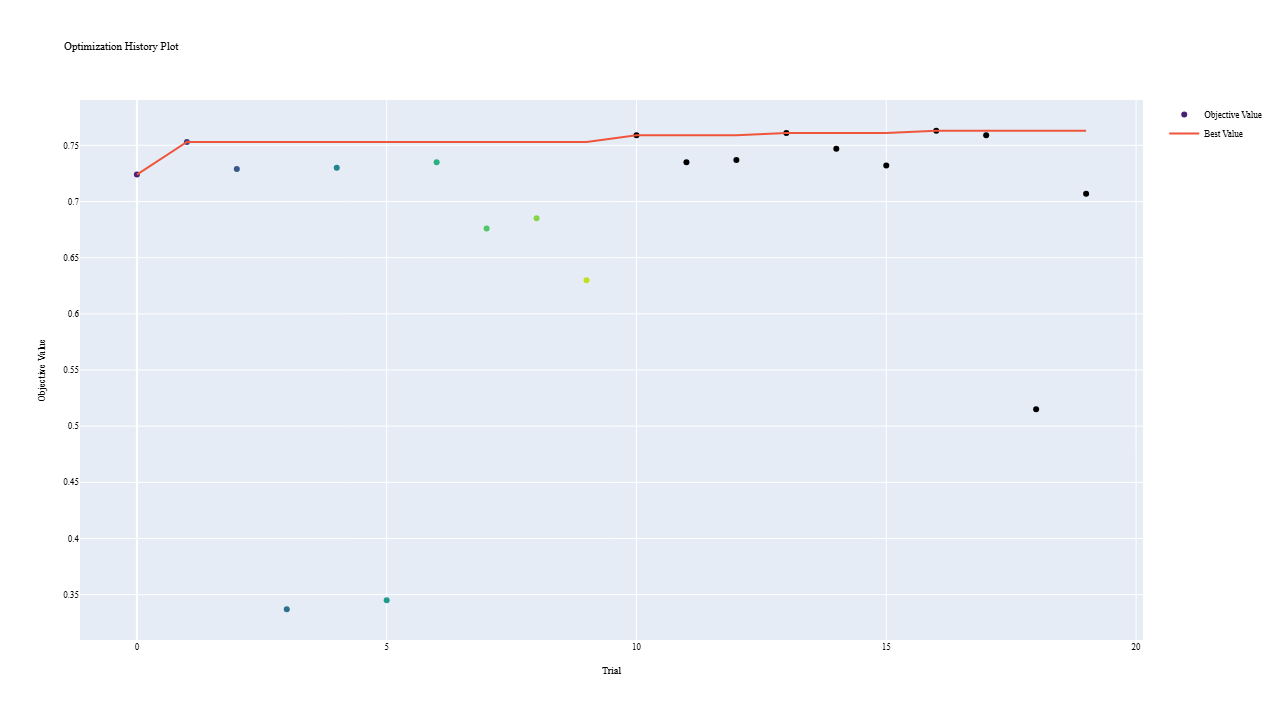
\includegraphics[width=\imagewidth, height=\imageheight, keepaspectratio]{optimization_history.png}
    \caption{Verlauf der Validierungsgenauigkeit über die Trials (je höher, desto besser).}

\end{figure}
\end{frame}


  \section{Ausblick}

\begin{frame}{Ausblick}
    quantitaiver Vergleich bayesian mit anderen methoden

    andere modelle

    etc
    
\end{frame}

%   \begin{frame}{Blocks}
%   Three different block environments are pre-defined and may be styled with an
%   optional background color.

%   \begin{columns}[T,onlytextwidth]
%     \column{0.5\textwidth}
%       \begin{block}{Default}
%         Block content.
%       \end{block}

%       \begin{alertblock}{Alert}
%         Block content.
%       \end{alertblock}

%       \begin{exampleblock}{Example}
%         Block content.
%       \end{exampleblock}

%     \column{0.5\textwidth}

%       \metroset{block=fill}

%       \begin{block}{Default}
%         Block content.
%       \end{block}

%       \begin{alertblock}{Alert}
%         Block content.
%       \end{alertblock}

%       \begin{exampleblock}{Example}
%         Block content.
%       \end{exampleblock}

%   \end{columns}
% \end{frame}

% \section{Second Section}
%   \begin{frame}{Second Frame}
%       The theme provides sensible defaults to
% \emph{emphasize} text, \alert{accent} parts
% or show \textbf{bold} results.
%   \end{frame}

%   \begin{frame}{References}
%   Some references to showcase [allowframebreaks] \cite{Knuth92,ConcreteMath,Simpson,Er01,greenwade93}
%   \cite{ConcreteMath}
% \end{frame}

% \begin{frame}{Animation}
%   \begin{itemize}[<+- | alert@+>]
%     \item \alert<4>{This is\only<4>{ really} important}
%     \item Now this
%     \item And now this
%   \end{itemize}
% \end{frame}

%___________________________________________________________________
\begin{frame}[label=conclusion, standout]
  Fragen?
\end{frame}

\appendix

%___________________________________________________________________
\begin{frame}{Literatur}
  \nocite{*}
  \printbibliography[heading=none]
\end{frame}

%___________________________________________________________________
\begin{frame}[allowframebreaks]{Wichtige Konzepte im Training}


\textbf{Regularisierung:}
\begin{itemize}
    \item \textbf{Dropout:} Deaktiviert zufällig Neuronen während des Trainings, um Overfitting zu reduzieren und die Generalisierung zu verbessern.
    \item \textbf{Weight Decay:} Fügt einen Strafterm für große Gewichte hinzu und verhindert dadurch übermäßig komplexe Modelle.
\end{itemize}

\textbf{Feature-Reduktion:}
\begin{itemize}
    \item \textbf{MaxPooling:} Verringert die räumliche Auflösung von Feature-Maps, indem pro Bereich nur der größte Aktivierungswert beibehalten wird.  
    Reduziert Rechenaufwand und sorgt für Translationstoleranz (robuster gegenüber kleinen Verschiebungen im Bild).
\end{itemize}

\textbf{Optimierung:}
\begin{itemize}
    \item \textbf{Adam:} Optimierer, der Momentum und RMSProp kombiniert. Passt die Lernrate adaptiv für jedes Gewicht an.
    \item \textbf{Learning Rate:} Schrittweite, mit der die Gewichte in Richtung des Gradienten aktualisiert werden.  
    Zu groß → instabil, zu klein → langsames Lernen.
\end{itemize}

\end{frame}

% \improve{bessere farbpalette parallel_coordinate}
%___________________________________________________________________
\begin{frame}
  \begin{figure}
    \centering
    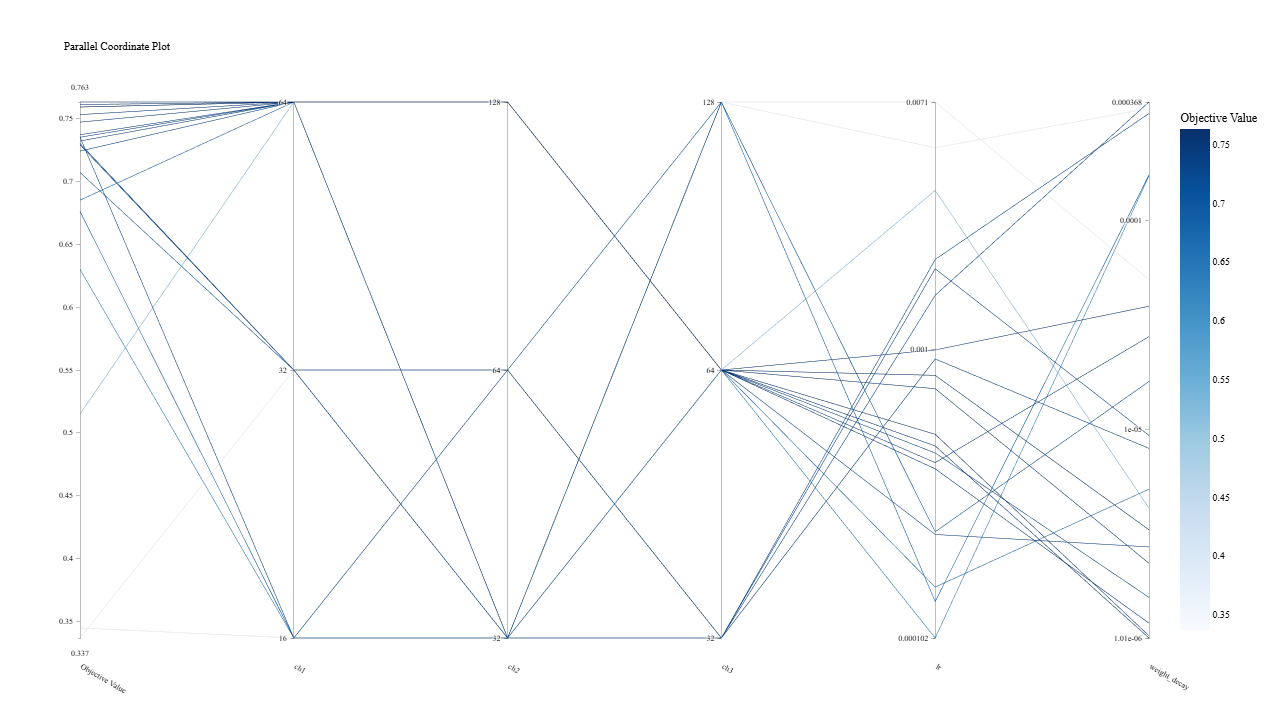
\includegraphics[width=\imagewidth, height=\imageheight, keepaspectratio]{parallel_coordinate.png}
  \end{figure}
\end{frame}

\end{document}